% !TeX spellcheck = en_GB
\documentclass[aspectratio=169]{beamer}

%\usepackage[utf8]{inputenc}
%\usepackage[T1]{fontenc}
%\usepackage{lmodern}
\usepackage{fontspec}
\usepackage[english]{babel}
\usepackage{amsmath}
\usepackage{amsfonts}
\usepackage{amssymb}
\usepackage{graphicx}
\usepackage{bigints}
\usepackage{verbatim}
\usepackage{caption}
\usepackage{mathtools}
\usepackage{physics}
\usepackage[export]{adjustbox}
\usepackage[backend=bibtex,style=numeric]{biblatex}
\usepackage{csquotes}

%\bibliography{String_Theory.bib}
\addbibresource{String_Theory.bib}

\usetheme{Madrid}

\usefonttheme{professionalfonts}

\setbeamertemplate{itemize item}[triangle]
\setbeamertemplate{itemize subsubitem}[square]
\setbeamertemplate{enumerate item}[default]
\setbeamertemplate{enumerate subitem}[default]
\setbeamertemplate{bibliography item}{\insertbiblabel}

\begin{document}	
	\author{Mate Zoltan Farkas}
	\title{An Introduction to String Theory}
	%\subtitle{}
	%\logo{}
	%\institute{}
	%\date{}
	%\subject{}
	\setbeamercovered{transparent}
	\setbeamertemplate{navigation symbols}{}
	
	\begin{frame}[plain]
		\maketitle
	\end{frame}
	
	\begin{frame}
		\frametitle{Table of Contents}
		\tableofcontents
	\end{frame}

%	\section{Introduction}
%	\subsection{Notation}
	
%	\begin{frame}
%		\frametitle{Introduction -- Notation}
%		\LARGE \color{red} Not necessary?
%		\color{black}
%		\begin{itemize}
%			\item Metric:
%			\begin{itemize}
%				\item $\eta_{\mu\nu}$ = diag(-1,+1, $\dots$, +1)
%			\end{itemize}
%			\item Products
%			\begin{itemize}
%				\item $X^2 = X^\mu X^\nu \eta_{\mu\nu}$
%			\end{itemize}
%		\end{itemize}
%	\end{frame}

	\section{The Relativistic Closed String}
	\subsection{The Relativistic Point Particle}
	
	\begin{frame}
		\frametitle{The Relativistic Point Particle -- The Action}
		\begin{itemize}[]
			\item<1-> Consider the action of a point particle (with fixed coordinates $X_\mu = (t,\vec{x})$ in a given frame):
			\begin{equation*}
				S = -m \int dt \, \sqrt{1-\dot{\vec{x}}\dot{\vec{x}}}
			\end{equation*}
			\item<1->[] $\rightarrow$ not Lorentz-invariant, due to mixture of spacial and temporal coordinates under a Lorentz-transformation $\Lambda$.
			\item[]
			\item<2-> Consider instead for a generalized coordinate $\tau$ along the line element:
			\begin{columns}
				\begin{column}{0.8\textwidth}
					\begin{equation*}
						S = -m \int d\tau \, \sqrt{-\frac{dX^\mu}{d\tau} \frac{dX^\nu}{d\tau}\eta_{\mu\nu}}
					\end{equation*}
				\end{column}
				\begin{column}{0.2\textwidth}
					\begin{figure}
						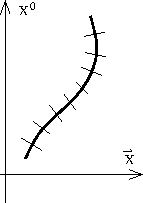
\includegraphics[width=0.5\linewidth]{res/TongP17_graph}
%						\caption*{Ref: \cite{tong_lectures_2012}}
					\end{figure}
				\end{column}
			\end{columns}
			\item[]<2-> Remark: $S$ is proportional to the integral over the worldline of the particle
		\end{itemize}
	\end{frame}

	\begin{frame}
		\frametitle{The Relativistic Point Particle -- Action Symmetries}
		\begin{itemize}
			\item[]<1-> What are the symmetries of
			\begin{equation*}
				S = -m \int d\tau \, \sqrt{-\frac{dX^\mu}{d\tau} \frac{dX^\nu}{d\tau}\eta_{\mu\nu}}
			\end{equation*}
			\item<2-> Reparametrization invariance:
			\begin{flushleft}
				Let $\tilde{\tau} = \tilde{\tau}(\tau)$. Then:
				\begin{equation*}
					S' = -m \int d\tilde{\tau} \, \sqrt{-\frac{dX^\mu}{d\tilde{\tau}}\frac{dX^\nu}{d\tilde{\tau}}\eta_{\mu\nu}} = S
				\end{equation*}
				$\rightarrow$ gauge symmetry of the action $\rightarrow$ still D-1 dof!
			\end{flushleft}
			\item<2-> Poincaré invariance:
			\begin{flushleft}
				Let:
				\begin{equation*}
					X'^\mu = \Lambda^\mu{}_\nu X^\nu + c^\mu
				\end{equation*}
				Then:
				\begin{equation*}
					S'=S, \qquad \text{as} \qquad \Lambda^\mu{}_\rho \, \eta_{\mu\nu} \, \Lambda^\nu{}_\sigma = \eta_{\rho\sigma}
				\end{equation*}
			\end{flushleft}
		\end{itemize}
	\end{frame}

	\subsection{Dynamics of a Relativistic String}
	\subsubsection{The Nambu-Goto Action}

	\begin{frame}[t]
		\frametitle{Dynamics of a Relativistic String -- The Nambu-Goto Action}
		Action of the Relativistic String?
		\begin{itemize}
			\item[]<only@1>
			\begin{center}
				\begin{tabular}{ccp{1.8cm}cc}
					particle & $\Leftrightarrow$ & worldline & $\Leftrightarrow$ & ${\displaystyle S = -m \int } \underbrace{d\tau \,\sqrt{-\frac{dX^\mu}{d\tau} \frac{dX^\nu}{d\tau}\eta_{\mu\nu}} }_{\text{line element }ds} $ \\[0.7cm]
					&&&&\\
					closed string & $\Leftrightarrow$ &\hphantom{worl} ? \hphantom{heet}& $\Leftrightarrow$ & ? \\
				\end{tabular}
			\end{center}
			\item[]<only@2>
			\begin{center}
				\begin{tabular}{ccp{1.8cm}cc}
					particle & $\Leftrightarrow$ & worldline & $\Leftrightarrow$ & ${\displaystyle S = -m \int d\tau \,\sqrt{-\frac{dX^\mu}{d\tau} \frac{dX^\nu}{d\tau}\eta_{\mu\nu}} }$ \\[0.7cm]
					&&&&\\
					closed string & $\Leftrightarrow$ & worldsheet & $\Leftrightarrow$ & ? \\
				\end{tabular}
			\end{center}
			\item[]<only@3>
			\begin{center}
				\begin{tabular}{ccp{1.8cm}cc}
					particle & $\Leftrightarrow$ & worldline & $\Leftrightarrow$ & ${\displaystyle S = -m \int d\tau \,\sqrt{-\frac{dX^\mu}{d\tau} \frac{dX^\nu}{d\tau}\eta_{\mu\nu}} }$ \\[0.7cm]
					&&&&\\
					closed string & $\Leftrightarrow$ & worldsheet & $\Leftrightarrow$ & Nambu-Goto/Dirac Action \\
				\end{tabular}
			\end{center}
			\item[]<3->
			\begin{columns}
				\begin{column}{0.8\textwidth}
					Boundary condition of closed strings living in $D$ dimensions:
					\begin{equation*}
					X^\mu(\tau,\sigma) = X^\mu(\tau,\sigma+2\pi) \quad  \text{for $\mu$} = 0,1,...,D-1; \, \sigma \in \left[0;2\pi\right)
					\end{equation*}
					Shorthand notation: $\sigma^\alpha = (\tau,\sigma)$ for $\alpha \in \{0;1\}$\\
				\end{column}
				\begin{column}{0.2\textwidth}
					\begin{figure}
						\centering
						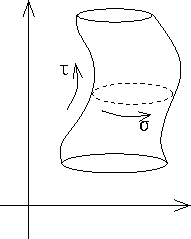
\includegraphics[width=\linewidth]{res/TongP21_graph}
%						\caption{}
%						\label{fig:tongp21graph}
					\end{figure}
					
				\end{column}
			\end{columns}
		\end{itemize}
	\end{frame}
	
	\begin{frame}
		\frametitle{Dynamics of a Relativistic String -- The Nambu-Goto Action}
		How to describe the surface area to construct the action?
		\begin{equation*}
			S \propto \int\displaylimits_{\partial V} d^2x = \int\displaylimits_{\partial V}d^2\sigma \left| \det J \right|
		\end{equation*}
		For this, first remember that any metric is given by:
		\begin{equation*}
			g_{\alpha\beta} = g(e_\alpha,e_\beta)
		\end{equation*}
		\color{black}
		So the metric on the worldsheet (the pullback metric) can be written as:
		\begin{equation*}
			\gamma_{\alpha\beta} = \underbrace{\frac{\partial X^\mu}{\partial\sigma^\alpha} \frac{\partial X^\nu}{\partial\sigma^\beta} \eta_{\mu\nu}}_{(J^T \eta J)_{\alpha\beta}}
		\end{equation*}
		Thus,
		\begin{equation*}
			\det \gamma = \det\eta \, (\det J)^2 = - (\det J)^2
		\end{equation*}
		\begin{equation*}
			\left| \det J \right| = \sqrt{-\det\gamma} = \sqrt{-\gamma}
		\end{equation*}
	\end{frame}

	\begin{frame}
		\frametitle{Dynamics of a Relativistic String -- The Nambu-Goto Action}
		So write the action as:
		\begin{equation*}
			S_{NG} = -\frac{1}{2\pi\alpha'} \int d^2\sigma \, \sqrt{-\gamma}
		\end{equation*}
		This action in invariant under,
		\begin{itemize}
			\item Poincaré transformations
			\item Reparametrization
		\end{itemize}
		and the eqations of motion (EoM) are given by:
		\begin{equation*}
			\partial_\alpha\left(\sqrt{-\gamma}\,\gamma^{\alpha\beta}\partial_\beta X^\mu\right) = 0
		\end{equation*}
		$\Rightarrow$ rather hard to quantize in this form! Alternatives?
	\end{frame}

	\subsubsection{The Polyakov Action}

	\begin{frame}
		\frametitle{Dynamics of a Relativistic String -- The Polyakov Action}
		Way out: \textbf{The Polyakov Action}:
		\begin{equation*}
			S_P = -\frac{1}{4\pi\alpha'}\int d^2 \, \sigma \sqrt{-g} \, g^{\alpha\beta}\,\partial_\alpha X^\mu \partial_\beta X^\nu \, \eta_{\mu\nu}
		\end{equation*}
		The EoMs:
		\begin{itemize}
			\item for $X^\mu$:
			\begin{itemize}
				\item same as for the Nambu-Goto action!
			\end{itemize}
			\begin{equation*}
				\partial_\alpha\left(\sqrt{-g}\,g^{\alpha\beta}\partial_\beta X^{\mu}\right) = 0
			\end{equation*}
			\item for $g_{\alpha\beta}$:
			\begin{equation*}
				g_{\alpha\beta} = 2 \frac{\partial_\alpha X^\mu \partial_\beta X^\nu \eta_{\mu\nu} }{g^{\rho\sigma}\partial_\rho X^\mu \partial_\sigma X^\nu \eta_{\mu\nu}} \equiv 2 \frac{\partial_\alpha X \partial_\beta X}{g^{\rho\sigma}\partial_\rho X \partial_\sigma X}
			\end{equation*}
		\end{itemize}
		Gains of the Polyakov action?
	\end{frame}

	\begin{frame}
		\frametitle{Dynamics of a Relativistic String -- The Polyakov Action}
		Symmetries of the Polyakov action
		\begin{equation*}
			S_P = -\frac{1}{4\pi\alpha'}\int d^2 \, \sigma \sqrt{-g} \, g^{\alpha\beta}\,\partial_\alpha X^\mu \partial_\beta X^\nu \, \eta_{\mu\nu}
		\end{equation*}
		\begin{itemize}
			\item Poincaré invariance
			\item Reparametrization invariance
			\item Invariance under:
			\begin{equation*}
				g'_{\alpha\beta} = \Omega^2(\sigma) g_{\alpha\beta}
			\end{equation*}
			$\Rightarrow$ \textbf{Weyl invariance}\\
			However, using the conformal gauge and writing $g$ as
			\begin{equation*}
				g_{\alpha\beta} = e^{2\phi}\eta_{\alpha\beta}
			\end{equation*}
			can be undone by a Weyl transformation ($\phi=0$). Thus,
			\begin{equation*}
				g_{\alpha\beta} = \eta_{\alpha\beta}
			\end{equation*}
%			\color{red} Plot of the transformation in action
		\end{itemize}
	\end{frame}

	\subsection{Equation of Motions from the Polyakov Action \& Classical Solutions}

	\begin{frame}
		\frametitle{The Polyakov Action -- Equation of Motion}
		With $g_{\alpha\beta} = \eta_{\alpha\beta}$ the EoMs
		\begin{equation*}
			\begin{cases}
				\partial_\alpha\left(\sqrt{-g}\,g^{\alpha\beta}\partial_\beta X^{\mu}\right) = 0 \\
				g_{\alpha\beta} =  2 \frac{\partial_\alpha X \partial_\beta X}{g^{\rho\sigma}\partial_\rho X \partial_\sigma X}
			\end{cases}
		\end{equation*}
		are reduced to:
		\begin{equation*}
			\begin{cases}
				\partial_\alpha\partial^\alpha X^{\mu} & = 0 \\
				T_{\alpha\beta} &= \partial_\alpha X \partial_\beta X - \frac{1}{2} \eta_{\alpha\beta} \eta^{\mu\nu} \partial_\mu X \partial_\nu X = 0
			\end{cases}
		\end{equation*}
		With the second constraints explicitly as:
		\begin{equation*}
			\begin{cases}
			T_{01} &= \dot{X}\cdot X' = 0 \\
			T_{00} &= T_{11} = \frac{1}{2} \left(\dot{X}^2 + X'^2 \right) = 0
			\end{cases}
		\end{equation*}
	\end{frame}	

	\begin{frame}
		\frametitle{The Polyakov Action -- Solution to the EoMs}
		To find a solution, define the lightcone coordinates as
		\begin{equation*}
			\sigma^\pm = \tau\pm\sigma
		\end{equation*}
		Then, the EoMs are given by
		\begin{equation*}
			\begin{cases}
				\partial_+\partial_-X^\mu &= 0 \\
				(\partial_+X)^2 &= 0 \qquad, \text{with} \, X^\mu(\tau,\sigma) = X^\mu(\tau,\sigma+2\pi) \\
				(\partial_-X)^2 &= 0 \\
			\end{cases}
		\end{equation*}
		\begin{align*}
			\Rightarrow X^\mu(\tau,\sigma) & = X^\mu_L(\sigma^+) + X^\mu_R(\sigma^-) \\
			X^\mu_{L}(\sigma^+) &= \frac{1}{2}x^\mu + \frac{1}{2} \alpha' p^\mu \sigma^+ + i\sqrt{\frac{\alpha'}{2}} \sum_{n\neq 0} \frac{1}{n} \tilde{\alpha}^\mu_n e^{-in\sigma^+} \\
			X^\mu_{R}(\sigma^-) &= \frac{1}{2}x^\mu + \frac{1}{2} \alpha' p^\mu \sigma^- + i\sqrt{\frac{\alpha'}{2}} \sum_{n\neq 0} \frac{1}{n} \alpha^\mu_n e^{-in\sigma^-} \\
		\end{align*}
	\end{frame}

	\begin{frame}
		\frametitle{The Polyakov Action -- Solution to the EoMs}
		The constraints $\left(\partial_\pm X\right)^2 = 0$:
		\begin{itemize}
			\item First:
			\begin{align*}
				\partial_- X^\mu = \frac{\alpha'}{2} p^\mu + \sqrt{\frac{\alpha'}{2}} \sum_{n\neq 0 } \alpha^\mu_n e^{-in\sigma^-} & \equiv \sqrt{\frac{\alpha'}{2}} \sum_{n} \alpha^\mu_n e^{-in\sigma^-} \\
				\text{with} \quad \alpha^\mu_0 & = \sqrt{\frac{\alpha'}{2}}p^\mu \\
			\end{align*}
			\item Then:
			\begin{align*}
				\left(\partial_-X\right)^2 &= \frac{\alpha'}{2} \sum_{n,p} \alpha_m \alpha_n e^{-i(n+m)\sigma^-}\\
				& = \alpha' \sum_n \underbrace{\frac{1}{2} \sum_m \alpha_m \alpha_{n-m}}_{L_n} e^{-in\sigma^-} \stackrel{!}{=} 0
			\end{align*}
		\end{itemize}
	\end{frame}

	\begin{frame}
		\frametitle{The Polyakov Action -- Solution to the EoMs}
		$\Rightarrow \infty$ number of constraints on $L_n$: 
		\begin{equation*}
			L_n = \tilde{L}_n = 0
		\end{equation*}
		However, $L_0$ contains the mass $M^2 = -p^2$ as:
		\begin{align*}
			L_0 &= \frac{\alpha'}{4}p^2 + \frac{1}{2} \sum_{m} \alpha_m \alpha_{-m} \\
			& \Rightarrow M^2 = \frac{4}{\alpha'} \sum_{m>0}\alpha_m\alpha_{-m} = \frac{4}{\alpha'} \sum_{m>0}\tilde{\alpha}_m\tilde{\alpha}_{-m}
		\end{align*}
		$\Rightarrow$ \textbf{Level matching}
	\end{frame}

	\begin{frame}
		\frametitle{Polyakov Action -- Summary}
		\begin{itemize}
			\item<1-> The Polyakov action
			\begin{equation*}
				S_P = -\frac{1}{4\pi\alpha'}\int d^2 \, \sigma \sqrt{-g} \, g^{\alpha\beta}\,\partial_\alpha X^\mu \partial_\beta X^\nu \, \eta_{\mu\nu}
			\end{equation*}
			gives rise to solutions in lightcone coordinates with left and right-moving modes:
			\begin{align*}
				X^\mu_{L;R}(\sigma^\pm) &= \frac{1}{2}x^\mu + \frac{1}{2} \alpha' p^\mu \sigma^\pm + i\sqrt{\frac{\alpha'}{2}} \sum_{n\neq 0} \frac{1}{n} \stackrel{(\textasciitilde)}{\alpha_n}{}^\mu e^{-in\sigma^\pm} 
			\end{align*}
			\item<2-> These modes have to fulfil the constraints of the action $\rightarrow$ level matching
			\begin{equation*}
				L_n = \tilde{L}_n = 0
			\end{equation*}
			\item<3-> They give the mass of the particle through:
			\begin{equation*}
				M^2 = \frac{4}{\alpha'} \sum_{m>0}\alpha_m\alpha_{-m} = \frac{4}{\alpha'} \sum_{m>0}\tilde{\alpha}_m\tilde{\alpha}_{-m}
			\end{equation*}
		\end{itemize}
	\end{frame}

	\section{Covariant Quantization of the  Classical Solutions}	

	\begin{frame}
		\frametitle{The Quantum String -- Covariant Quantization}
		First, promote $X^\mu$ and $\Pi^\mu = 1/2\pi\alpha' \dot{X}^\mu$ to operators with the usual commutators:
		\begin{equation*}
			\left[X^\mu(\tau,\sigma), \Pi^\nu(\tau,\sigma')\right] = i\delta(\sigma'-\sigma)\delta^{\mu\nu}
		\end{equation*}
		Then:
		\begin{align*}
			\left[x^\mu,p_\nu\right] &= i\delta^\mu_\nu \\
			\left[\alpha^\mu_n, \alpha^\nu_m\right] = \left[\tilde{\alpha}^\mu_n, \tilde{\alpha}^\nu_m\right] &= n \eta^{\mu\nu} \delta_{n,-m}
		\end{align*}
		Introduce the creation operators as
		\begin{equation*}
			a_n = \frac{\alpha_n}{\sqrt{n}}, \quad a^\dagger_n = \frac{\alpha_{-n}}{\sqrt{n}}, \quad n>0
		\end{equation*}
		which gives the usual
		\begin{equation*}
			\left[a_n,a^\dagger_m\right] = \delta_{nm}
		\end{equation*}
		$\Rightarrow$ construction of the Fock space!
	\end{frame}

	\begin{frame}
		\frametitle{The Quantum String -- Covariant Quantization}
		$1^{st}$ problem with this approach: appearance of ghosts, due to the relation:
		\begin{equation*}
			\left[\alpha^\mu_n, \alpha^\nu_m\right] = n \eta^{\mu\nu} \delta_{n,-m} \quad \rightarrow \quad \text{negative norms for } \mu=\nu=0 \quad \rightarrow \quad \text{ghosts (unphysical)}
		\end{equation*}
		$2^{nd}$ problem: What about the constraints $L_n = \tilde{L}_n = 0$? How to order the operators in $L_n$?
		\begin{itemize}
			\item one could require for any physical state $\ket{\varphi}$:
			\begin{align*}
				&\qquad \bra{\phi}L_n\ket{\varphi} = \bra{\phi}\tilde{L}_n\ket{\varphi} = 0 \\
				& \Rightarrow L_n\ket{\varphi} = 0, \, n>0 \quad (L^\dagger_n = L_{-n}) \\
			\end{align*}
			\item For $L_0$:
			\begin{align*}
				 \qquad L_0 = \sum_{m=1}^{\infty} \alpha_{-m} \alpha_m + \frac{1}{2} &\alpha^2_0 \\
				 \Rightarrow (L_0 - a)\ket{\varphi} = 0 \quad & \rightarrow \quad  M^2 = \frac{4}{\alpha'} \left(-a+\sum_{m=1}^{\infty}\alpha_{-m}\alpha_m\right) \\
			\end{align*}
		\end{itemize}
	\end{frame}

	\section{Quantization in the Lightcone Gauge}
	
	\begin{frame}
		\frametitle{The Quantum String -- Quantization in the Lightcone Gauge}
		To resolve these problems, introduce lightcone coordinates:
		\begin{align*}
			X^\pm = \sqrt{\frac{1}{2}} \left(X^0\right.&\left.\pm X^{D-1}\right)
%			\Rightarrow ds^2 = -2\cdot dX^+dX^- &+ \sum_{i=1}^{D-2}dX^idX^i
		\end{align*}
		and solve the EoMs $\left(\partial_+\partial_-X^\mu = 0, \quad (\partial_+X)^2 = 0, \quad (\partial_-X)^2 = 0 \right)$  in the lightcone gauge: 
		\begin{equation*}
%			\begin{cases}
			X^+ = x^+ + \alpha'p^+ \tau = \underbrace{\frac{1}{2}x^+ + \frac{1}{2} \alpha' p^+ \sigma^+}_{X^+_L(\sigma^+)} + \underbrace{\frac{1}{2}x^+ + \frac{1}{2} \alpha' p^+ \sigma^-}_{X^+_R(\sigma^-)}
%			\end{cases}
		\end{equation*}
		Solution for $X^-$:
		\begin{align*}
			X^-_L(\sigma^+) &= \frac{1}{2}x^- + \frac{1}{2} \alpha' p^- \sigma^+ + i \sqrt{\frac{\alpha'}{2}} \sum_{n\neq 0} \frac{1}{n}\tilde{\alpha}^-_n e^{-in\sigma^+}\\
			X^-_R(\sigma^-) &= \frac{1}{2}x^- + \frac{1}{2} \alpha' p^-\sigma^- + i \sqrt{\frac{\alpha'}{2}} \sum_{n\neq 0} \frac{1}{n}\alpha^-_n e^{-in\sigma^-} \\
		\end{align*}
	\end{frame}

	\begin{frame}
		\frametitle{The Quantum String -- Quantization in the Lightcone Gauge}
		Now, the oscillator modes $\alpha^-_n$:
		\begin{equation*}
			\alpha_n^- = \sqrt{\frac{1}{2\alpha'}} \frac{1}{p^+} \sum_{m=-\infty}^{m=+\infty}\sum_{i=1}^{D-2}\alpha^i_{n-m}\alpha^i_m
		\end{equation*}
		And, the level matching condition becomes:
		\begin{equation*}
			M^2 = \frac{4}{\alpha'} \sum_{i=1}^{D-2}\sum_{n>0}^{}\alpha^i_{-n}\alpha^i_n = \frac{4}{\alpha'} \sum_{i=1}^{D-2}\sum_{n>0}^{}\tilde{\alpha}^i_{-n}\tilde{\alpha}^i_n 
		\end{equation*}
		Gain: we have 2(D-2) oscillator modes with spacial indices only\\
		$\qquad \Rightarrow$ after quantization we only have positive norms, due to
		\begin{equation*}
			\left[\alpha^i_n,\alpha^j_m\right]=\left[\tilde\alpha^i_n,\tilde\alpha^j_m\right] = n\delta^{ij}\delta_{n,-m}
		\end{equation*}
		$\Rightarrow$ 1$^{\text{st}}$ problem solved.
	\end{frame}

	\begin{frame}
		\frametitle{The Quantum String -- Quantization \& Constraints}
		What about the mass spectrum and the ordering ambiguity?\\
		Take the classical result and swap the operators using the commutator 			$\left[\alpha^i_n,\alpha^j_{-m}\right]= n\delta^{ij}\delta_{n,m}$
		\begin{equation*}
			M^2 = \frac{4}{\alpha'} \left(\frac{1}{2}\sum_{i=1}^{D-2}\sum_{n\neq 0}^{}\alpha^i_{-n}\alpha^i_n -a \right) = \frac{4}{\alpha'} \left(\sum_{i=1}^{D-2}\sum_{n>0}\alpha^i_{-n}\alpha^i_n+\frac{D-2}{2}\sum_{n>0}n\right)
		\end{equation*}
		Interpreting the term $\sum n$:
		\begin{align*}
			\sum_{n>0}n &= \lim_{\epsilon\rightarrow 0} \sum_{n>0}ne^{-\epsilon n} = -\frac{\partial}{\partial\epsilon}\sum_{n>0}e^{-\epsilon n} = \\
			& = -\frac{\partial}{\partial\epsilon} (1-e^{-\epsilon})^{⁻1} = \frac{1}{\epsilon^2}-\frac{1}{12}+O(\epsilon)
		\end{align*}
		After renormalization: $\sum n = -\frac{1}{12}$ \quad $\Rightarrow$ \quad $a=-(D-2)/24$
	\end{frame}

	\begin{frame}
		\frametitle{The Quantum String -- The Critical Dimension}
		What is the value $D$?
		\begin{itemize}
			\item No excitations are present: ground state with
			\begin{columns}
				\begin{column}{0.6\linewidth}
			\begin{equation*}
				M^2 = -\frac{1}{\alpha'}\frac{D-2}{6} \quad < 0
			\end{equation*}
			\end{column}
			\begin{column}{0.4\linewidth}
				\begin{figure}
%					\centering
					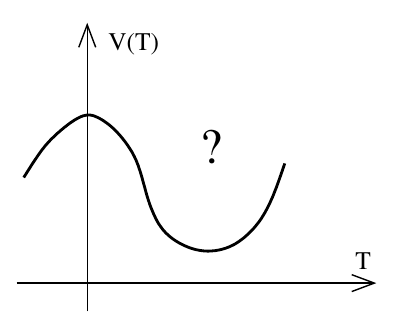
\includegraphics[width=0.4\linewidth]{res/tachyon}
%					\caption{}
%					\label{fig:tachyon}
				\end{figure}
				
			\end{column}
			\end{columns}
			$\rightarrow$ Tachyons: the string sits at an unstable point in the tachyon field; not well understood
			\item First excitations $\tilde{\alpha}^i_{-1}\alpha^j_{-1}\ket{0;p}$ yield:
			\begin{equation*}
				M^2 = \frac{4}{\alpha'}\left(1-\frac{D-2}{24}\right)
			\end{equation*}
			with $(D-2)^2$ degrees of freedom (dof). However, in the rest frame of the particle there are $(D-1)^2$ dof $\rightarrow$ no rest frame $\rightarrow M^2=0$
			\[\rightarrow D=26\]
		\end{itemize}
	\end{frame}


	\begin{frame}
		\frametitle{The Graviton}
		The states $\tilde{\alpha}^i_{-1}\alpha^j_{-1}\ket{0;p}$ transform in the 24 $\otimes$ 24 representation of SO(24), which decomposes into:
		\begin{equation*}
			24 \otimes 24 = \underbrace{\text{traceless symmetric}}_{\text{massless spin 2-particle}} \oplus \underbrace{\text{anti-symmetric}}_{\text{Kalb-Ramond field $B_{\mu\nu}$}} \oplus \underbrace{\text{ singlet}}_\text{{dilaton}}
		\end{equation*}
		Feynman and Weinberg:\\
		\begin{itemize}
			\item[] Given a massless, spin 2 particle. Then, it must be invariant at linearized level under
			\begin{equation*}
				h_{\mu\nu} \rightarrow h_{\mu\nu} + \partial_\mu\xi_\nu + \partial_\nu\xi_\mu
			\end{equation*}
			to avoid negative norm states, and it should be present in interactions. This is only possible if the theory obeys diffeomorphism invariance $\rightarrow$ General Relativity
		\end{itemize}
	\end{frame}

	\section{Open Strings and D-Branes}
	
	\begin{frame}
		\frametitle{Open Strings -- Action and Boundary Conditions}
		\begin{columns}
			\begin{column}{0.6\textwidth}
						Open strings are described by the Polyakov action:
				\begin{equation*}
				S = -\frac{1}{4\pi\alpha'} \int d^2\sigma \, \partial_\alpha X \partial^\alpha X \qquad \sigma \in [0,\pi]
				\end{equation*}
				which under variation yields
			\end{column}
			\begin{column}{0.4\textwidth}
				\begin{figure}
					\centering
					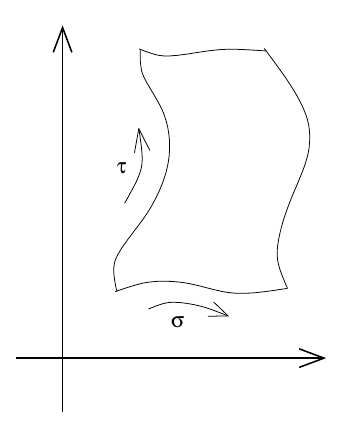
\includegraphics[width=0.5\linewidth]{res/open_string}
%					\caption{}
%					\label{fig:openstring}
				\end{figure}
				
			\end{column}
		\end{columns}
		\begin{equation*}
			\delta S = \frac{1}{2\pi\alpha'} \cdot \int_{\tau_i}^{\tau_f} \, d\tau \int_{0}^{\pi}\, d\sigma (\partial_\alpha \partial^\alpha X)\delta X + \underbrace{\left.\int_{0}^{\pi} \, d\sigma \dot{X} \delta X\right|^{\tau_f}_{\tau_i}}_{ = 0 } - \underbrace{ \left. \int_{\tau_i}^{\tau_f} d\tau \, X' \delta X \right|^\pi_0}_{\stackrel{!}{=} 0 }
		\end{equation*}
		\begin{columns}
			\begin{column}{0.6\textwidth}
		\begin{itemize}
			\item Neumann conditions: moving ends ($\delta X \neq 0$)
				\begin{equation*}
					\partial_\sigma X  = 0 \quad \text{for} \, \sigma = 0,\pi
				\end{equation*}
		\end{itemize}
		\end{column}
		\begin{column}{0.4\textwidth}
			\begin{itemize}
				\item Dirichlet conditions: fixed ends
			\begin{equation*}
				\delta X  = 0 \quad \text{for} \, \sigma = 0,\pi
			\end{equation*}
		\end{itemize}
		\end{column}
		\end{columns}
	\end{frame}

	\begin{frame}
		\frametitle{Open Strings -- Dp-Branes}
		\begin{itemize}
			\item Quantization: regular mode expansion + lightcone gauge
			\begin{columns}
				\begin{column}{0.6\textwidth}
					\begin{align*}
					X^\mu_{L}(\sigma^+) &= \frac{1}{2}x^\mu + \alpha' p^\mu \sigma^+ + i\sqrt{\frac{\alpha'}{2}} \sum_{n\neq 0} \frac{1}{n} \tilde{\alpha}^\mu_n e^{-in\sigma^+} \\
					X^\mu_{R}(\sigma^-) &= \frac{1}{2}x^\mu + \alpha' p^\mu \sigma^- + i\sqrt{\frac{\alpha'}{2}} \sum_{n\neq 0} \frac{1}{n} \alpha^\mu_n e^{-in\sigma^-} \\
					\end{align*}
				\end{column}
				\begin{column}{0.4\textwidth}
					\begin{equation*}
					X^\pm = \sqrt{\frac{1}{2}}\left(X^0 \pm X^p \right)
					\end{equation*}
				\end{column}
			\end{columns}
			\item Dirichlet boundary conditions fix ends, i.e. for
			\begin{columns}
				\begin{column}{0.6\textwidth}
					\begin{align*}
						\partial_\sigma X^a &= 0 \qquad \text{for } a=0,...,p \\
					X^I &= c^I \qquad \text{for } I=p+1,...,D-1
					\end{align*}
					we have 2 endpoints moving freely on a (p+1)-dimensional hypersurface = \textbf{Dp-brane}
				\end{column}
				\begin{column}{0.4\textwidth}
					\begin{figure}
						\centering
						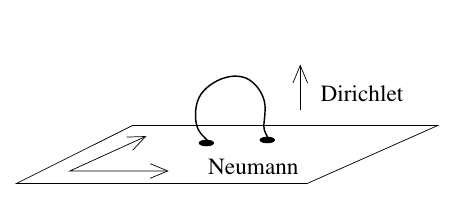
\includegraphics[width=0.7\linewidth]{res/boundary}
					\end{figure}	
				\end{column}
			\end{columns}
		\end{itemize}
	\end{frame}

	\begin{frame}
		\frametitle{Bosonic States -- Mass Spectrum}
		\begin{itemize}
			\item Mass spectrum:
			\begin{equation*}
				M^2 = \frac{1}{\alpha'} \left( \underbrace{ \sum_{i=1}^{p-1}\sum_{n>0} \alpha^i_{-n}\alpha^i_{n}}_{\text{longitudinal oscillations}} + \underbrace{\sum_{i=p+1}^{D-1}\sum_{n>0} \alpha^i_{-n}\alpha^i_{n}}_{\text{transversal oscillations}} + \frac{2-D}{24} \right)
			\end{equation*}
		\end{itemize}
			\begin{columns}
			\begin{column}{0.7\textwidth}
				\begin{itemize}
				\item The ground state: $M^2 = - \frac{1}{\alpha'}$
					\begin{itemize}
						\item tachyonic
						\item interpretation: unstable brane decaying into closed strings
					\end{itemize}
				\end{itemize}
				\end{column}
				\begin{column}{0.3\textwidth}
					\begin{figure}
						\centering
						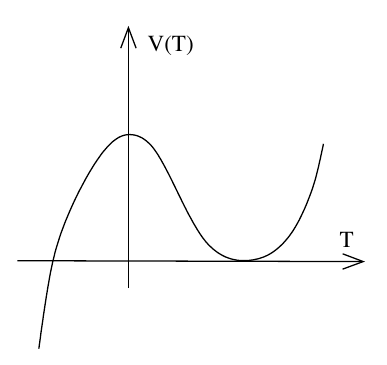
\includegraphics[width=0.7\linewidth]{res/tachyon_zero}
%						\caption{}
%						\label{fig:tachyonzero}
					\end{figure}
					
				\end{column}
			\end{columns}
	\end{frame}

	\begin{frame}
		\frametitle{Bosonic States -- Mass Spectrum}
		\begin{itemize}
			\item The first excited states:
			\begin{itemize}
				\item $M^2 = 0 \rightarrow$ massless
				\item Longitudinal oscillations:
				\begin{equation*}
					\alpha^a_{-1}\ket{0;p} \qquad a = 1,...,p-1
				\end{equation*}
				Spin 1 particles living in the brane $\rightarrow$ photon
				\item Transverse oscillations:
				\begin{equation*}
					\alpha^I_{-1}\ket{0;p} \qquad I = p+1,...,D-1
				\end{equation*}
				hints the dynamics of the brane\\
				\quad $\rightarrow$ string theory = string + brane dynamics!
			\end{itemize}
		\end{itemize}
	\end{frame}

	\begin{frame}
		\frametitle{Conclusion}
		\begin{itemize}
			\item Strings are described by the Polyakov action
			\item Both theories require $D=26$ to sustain Lorentz-invariance
			\begin{itemize}
				\item Closed Strings:
				\begin{itemize}
					\item Constraints imply the level-matching conditions $L_n = \tilde{L_n} = 0$
					\item Solutions can be quantized in the lightcone gauge $\rightarrow \, \alpha_n$
					\item Imply a massless spin 2 particle
				\end{itemize}
				\item Open Strings:
				\begin{itemize}
					\item Dynamics constrained by Dirichlet and Neumann boundary conditions
					\item Imply massless spin 1 particles
				\end{itemize}
			\end{itemize}
		\end{itemize}
	\end{frame}

	\begin{frame}
		\frametitle{Further Reading}
		\printbibliography
	\end{frame}

\end{document}